\chapter{流式主题模型的采样算法}
\label{chapter:sample}
Gibbs采样算法是LDA模型估计参数的一种主要方法。
本文提出的流式主题模型也是基于Gibbs采样设计的。
流式数据环境对算法的实时性要求很高。对于一批数据的处理,如果时间过长,有可能造成超时,数据堆积等等不稳定因素。
一般的Gibbs采样的复杂度与主题模型的主题个数有关,每次采样的时间复杂度为O($K$)。
当$K$值太大时,采样的效率会遭受到极大的影响。为了保证算法效率,以及维持系统的稳定性,O($K$)的采样算法显然是无法被接受的。
好在许多地方都提到了一些更快的采样方法。接下来本文将主要介绍如何设计更高效的采样算法。

\section{MCMC简介}
统计采样是个很常见的问题,通常在进行采样之前,我们都需要知道采样的来自的具体分布。但是,也有很多时候采样的分布的概率形式非常复杂,或者很难计算得到。
因而通过计算概率分布之后再进行统计采样的的方法也会遇到困难。
MCMC(Markov Chain Monte Carlo, MCMC)方法是解决这种问题的常见途径。

\begin{theorem}[马氏链收敛定理]
如果一个非周期马氏链具有转移概率矩阵$P$, 且任何状态是连通的,那么有:

1. $\lim_{n\rightarrow \infty} P_{ij}^n = \pi(j)$

2. $\pi(j) = \sum_{i = 0}^{\infty}{\pi(i)P_{ij}}$

3. $\pi$是方程$\pi P = \pi$的唯一非负解

4. $\sum_{i=0}^{\infty}{\pi_i} =  1$

称分布$\pi$为马氏链的平稳分布。

\end{theorem}

从任何初始概率分布$\pi_0$出发,我们在马氏链上做状态转移,记$X_i$的概率分布为$\pi_i$,则有:
\begin{align*}
X_0 \sim \pi_0(x) \\
X_1 \sim \pi_1(x) \\
... \\
X_n \sim \pi_n(x) = \pi(x) \\
X_{n+1} \sim \pi(x) \\
X_{n+2} \sim \pi(x) \\
\end{align*}

由马氏链收敛定理,概率分布$\pi_i(x)$将收敛到平稳分布$\pi(x)$。假设到第$n$步的时候马氏链收敛,我们得到$X_n, X_{n+1}, X_{n+2}, ... \sim \pi(x)$是服从于同一个分布的随机变量。
那么如果从一个具体的初始状态$x_0$开始,沿着马氏链按照概率转移矩阵做跳转,
那么我们得到一个转移序列$x_0, x_1, x_2, ..., x_n , x_{n+1}, ...$,由于马氏链的收敛行为,我们知道$x_n, x_{n+1}, ...$都是来自于平稳分布$\pi(x)$的观测值。
使用这个绝妙的方法,我们便得到了一组来自于$\pi(x)$分布的样本。

\subsection{Metropolis-Hastings采样}
根据上面的介绍,我们知道了在马氏链收敛定理中一个很关键的因素便是转移矩阵$P$,所以MCMC的一个关键问题便是如何定义和构造转移矩阵$P$,使得我们能够得到平稳的分布$\pi(x)$。

\begin{theorem}[细致平稳条件]
如果非周期马氏链的转移矩阵$P$和分布$\pi(x)$满足
\begin{equation}
\pi(i) P_{ij} = \pi(j) P_{ji}\mbox{  for all }i,j
\end{equation}
\end{theorem}

显然根据上面的细致平稳条件,我们很容易得出:
\begin{align*}
\sum_{i=1}^{\infty}{\pi(i) P_{ij}} = \sum_{i=1}^{\infty}{\pi(j) P_{ji}}= \pi(j) \Rightarrow \pi P = \pi
\end{align*}

给定非周期马氏链以及概率分布$p(x)$,现在假设已经得到了一个转移矩阵$Q$,用$q(i \rightarrow j)$表示从状态$i$转移到状态$j$的概率,
通常细致平稳条件并不成立:
\begin{align*}
p(i)q(i\rightarrow j) \neq p(j) q(j \rightarrow i)
\end{align*}

为了得到快速得到一个满足细致平稳条件的马氏链,我们对原来的马氏链做一些修改。
比如,引入接受概率$\alpha(i -> j)$使得
\begin{equation}
\label{eq:accept}
p(i) \underbrace{q(i \rightarrow j) \alpha(i \rightarrow j)}_{q^{\prime}(i \rightarrow j)}= p(j) \underbrace{q( j \rightarrow i ) \alpha(j \rightarrow i)}_{q^{\prime}(j \rightarrow i)}
\end{equation}
为了使得式\ref{eq:accept}成立,最简单的方式便是令
\begin{align*}
\alpha(i \rightarrow j ) = p(j)q(j \rightarrow i), \alpha(j \rightarrow i) = p(i) q(i \rightarrow j)
\end{align*}

通过上面改造,我们顺利得到了一个满足细致平稳条件的新的非周期马氏链,令其转移矩阵为$Q^{\prime}$。因此马氏链$Q^{\prime}$的平稳分布便是$p(x)$。
这个过程可以通俗地理解为在原来的马氏链$Q$上,从状态$i$以概率$q(i \rightarrow j)$转移到状态$j$需要通过接受概率$\alpha(i \rightarrow j)$。
因而,$q(i \rightarrow j)$也被称为提议分布。

尽管如此,我们发现目前接受概率被定义为两个概率的乘积,可想而知得到的接受概率$\alpha(i \rightarrow j)$会是一个比较小的小数,那么有很大的概率会转移失败。
如果失败太多次的话,会严重影响收敛到平稳分布的速度。

为此我们可以同比放大两边的接受概率而不破坏细致平稳条件,令:
\begin{equation}
\alpha(i \rightarrow j) = \min\left\{ \dfrac{p(j)q(j \rightarrow i)}{p(i)q(i \rightarrow j)},1 \right\}
\end{equation}

于是经过上面的改造,我们得到一个接受概率较大的又满足细致平稳条件的马氏链。
这种做法被称为Metropolis-Hastings采样算法\ref{alg:metropolis-hasting}
\begin{algorithm}[htb]  
\caption{Metropolis-Hastings Sampling} 
\label{alg:metropolis-hasting} 
\begin{algorithmic}[1] 
\State Set initial state of markov chain $X_0 = x_0$
\For{t = 0, 1, 2, ...}
\State Sample $y \sim q(x_t \rightarrow y)$
\State Sample $u \sim Uniform[0,1]$
\State Set $\alpha( x_t \rightarrow y) = \min \left\{ \dfrac{p(x_t)q(y \rightarrow x_t)}{p(y)q(x_t \rightarrow y)}, 1\right\}$
\If{$u < \alpha(x_t \rightarrow y)$}
\State Accept $x_t \rightarrow y$
\Else
\State Reject $x_t \rightarrow y$
\EndIf
\EndFor
\end{algorithmic}  
\end{algorithm}  

\subsection{Gibbs采样}
Gibbs采样对应于高维的情形。根据高维概率分布的特性,我们能直接找到满足细致平稳条件的概率转移矩阵。

不妨先来讨论二维的情形,假设存在一个二维的概率分布$p(x, y)$,考察$x$轴坐标相同的两个点$A(x, y_1), B(x, y_2)$,我们会发现如下性质:
\begin{align*}
p(x, y_1) p(y_2 | x) = p(x) p(y_1| x) p(y_2 |x )\\
p(x, y_2) p(y_1 | x) = p(x) p(y_2| x) p(y_1 |x )\\
\end{align*}
所以得到
\begin{align*}
p(x, y_1) p(y_2 | x) = p(x, y_2) p(y_1 | x) \\
\Rightarrow p(A) p(y_2|x) = p(B) p(y_1 | x)
\end{align*}

根据上面的特性,给定分布$p(x,y)$,如果固定$x$轴,并且以概率$p(y | x)$作为转移概率,这时候任意两点之间转移满足细致平稳条件。同理固定$y$轴时也得到一样的结论。
因此,我们可以构造一个转移概率矩阵Q使得:
\begin{align*}
& Q(A \rightarrow B) = p(y_B | x), & if~~x_A = x_B = x \\
& Q(A \rightarrow C) = p(x_C | y), & if~~y_A = y_C = y \\
& Q(A \rightarrow D) = 0, & otherwise
\end{align*}

如算法\ref{alg:gibbs-sampling},马氏链的转移是按照坐标轴下降的方式串行地进行转移。等待马氏链收敛之后,我们便能够得到样本的分布$p(x,y)$,在收敛之前的阶段成为burn-in阶段。

\begin{algorithm}[htb]  
\caption{2-Dimension Gibbs Sampling}
\label{alg:gibbs-sampling}
\begin{algorithmic}[1] 
\State Set initial state of markov chain $X_0 = x_0, Y_0 = y_0$
\For{t = 0, 1, 2, ...}
\State Sample $y_{t+1} \sim p(y | x_t)$
\State Sample $x_{t+1} \sim p(x | y_{t+1})$
\EndFor
\end{algorithmic}  
\end{algorithm}  

\section{主题模型采样算法}
前面的章节已经简略地介绍了主题模型的Gibbs采样参数估计方法。
在LDA模型中我们会关心主题变量$z$在语料上的分布,然而我们事先并不知道$p\mathbf{ (z, w)}$的具体情况。
我们已经知道了通过MCMC方法可以收敛得到一些来自于某一稳定分布的样本。
为了应用MCMC来对LDA模型中的主题变量进行抽样,关键问题在于如何构建非周期性马氏链。
\begin{equation}
\label{eq:stable-cond}
p(z_i = x , \mathbf{z}_{\neg i}, \mathbf{w}) p( z_i = y | \mathbf{z}_{\neg i},  \mathbf{w})  =  
p(z_i = y , \mathbf{z}_{\neg i}, \mathbf{w}) p( z_i = x | \mathbf{z}_{\neg i},  \mathbf{w}) 
\end{equation}

根据公式\ref{eq:stable-cond},令$p( z_i = k | \mathbf{z}_{\neg i},  \mathbf{w})$为第$i$维的变量状态之间的转移概率,
那么在这个维度上各个状态之间的转换满足细致平稳条件。
现假设,LDA模型某一轮迭代的输入语料中有$M$个文档,文档的平均长度为$\bar{L}$,主题模型设定的主题变量个数为$K$。
只需要将算法\ref{alg:gibbs-sampling}扩展到更高维(语料维度$M \times \bar{L}$),便得到了常见的LDA Gibbs采样算法。
那么LDA模型迭代一轮的时间复杂度为$O(M\times \bar{L} \times K)$,其中一次采样的复杂度为$O(K)$。
也就是说,随着主题模型变量个数的增大,模型的时间消耗随着线性增长。这种采样复杂度的效率较低。
实际上,利用主题模型参数的稀疏性,采样算法的时间和空间复杂度都会得到降低。
本文在本节的以下部分介绍几种高效的采样算法。

\subsection{Sparse LDA}
在此之前,本文已经多次介绍了LDA主题模型的采样公式:
\begin{equation}
\label{eq:sample-prob}
p( z_i = k | \mathbf{z}_{\neg i},  \mathbf{w}) 
	\propto  \dfrac{ n_{k, w_i}^{\neg di} + \eta }{ n_{k, \cdot}^{\neg di} + V\eta}(n_{k,d}^{\neg di} + \alpha)
\end{equation}

本文将式子\ref{eq:sample-prob}右式看做主题$z=k$的权重,表示为$q(z = k)$。
那么对该概率分布进行采样,就要计算右式的总和$\sum_k{q(z = k)}$,然后选取随机数$u \sim U(0, \sum_k{q(z= k)}$,
再找到$t$使得$\sum_k^{t-1}{q(z=k)} < u <= \sum_k^{t}{q(z=k)}$。
但事实上,给定任意词汇$q(z=k)$都是稀疏的,大部分权重只会被分配给部分的主题。
Sparse LDA从稀疏性的角度出发,从新审视了抽样概率\ref{eq:sample-prob},将式子展开会得到如下公式:
\begin{equation}
\label{eq:sparse-sample-prob}
p( z_i = k | \mathbf{z}_{\neg i},  \mathbf{w}) 
	\propto  \dfrac{\alpha \eta }{ n_{k, \cdot}^{\neg di} + V\eta} + 
	\dfrac{ n_{k, m}^{\neg di} \eta }{ n_{k, \cdot}^{\neg di} + V\eta} +
	\dfrac{ n_{k, w_i}^{\neg di} (n_{k, m}^{\neg di} + \alpha)}{ n_{k, \cdot}^{\neg di} + V\eta}
\end{equation}
不难发现,其中第一项是一个常数项,第二项与当前的词汇$w_i$无关,第三项也是一个相对稀疏的项。
根据上面的分解,我们可以得到$\sum_k{q(z=k)}$的分解公式:
\begin{align}
s =& \sum_k {  \dfrac{\alpha \eta }{ n_{k, \cdot}^{\neg di} + V\eta}}\\
r =& \sum_k {\dfrac{ n_{k, m}^{\neg di} \eta }{ n_{k, \cdot}^{\neg di} + V\eta}}\\
q =& \sum_k {\dfrac{ n_{k, w_i}^{\neg di} (n_{k, m}^{\neg di} + \alpha)}{ n_{k, \cdot}^{\neg di} + V\eta}}
\end{align}
上面的式子将一个完全的采样分布$q(z)$分割为三个部分。之前的采样等价于$u \sim U(0, s + r + q)$。
如果$u \le s$,那么采样只使用到了平滑项,因为该项不会发现变化,因此可以预先计算好权重,在采样时只需要$O(1)$的复杂度便可以得到结果;
如果$s < u \le r $,那么只使用第二项,对于该项的权重计算仅需要遍历所有的$ n_{k, m}^{\neg di} \ne 0$的项,一个文档通常只会集中表达若干个主题,因此$O(K_d) << K$;
最后如果$ u > (s + r) $,则使用到了第三项,对于该项的权重计算仅需要遍历所有的$ n_{k, w}^{\neg di}\ne 0 $的项,同样一个词汇的语义集中于若干个主题,因此$O(K_w) << K$。

在实际计算过程中,我们会发现$r$只与文档的主题计数有关,每个文档出现时只需要进行一次$r$的计算,在文档内部遍历时持续的使用常数时间来更新即可。
然而每个文档每次词出现都需要重新计算一次$q$,并且由于$\alpha, \eta$的值较小,$s, r << q$,所以绝大多数的采样最终会落在$q$之上。
也就是说真正影响该算法效率的项是$q$,总的来说这个方法的模型复杂度基本服从$O(K_w)$,相对于原先的$O(K)$复杂度有了大大的提升。
Sparse LDA为了提高算法效率,还针对$q$提出了一些缓存和优化策略,但是这些方法的提升空间都很有限,并且需要消耗大量的存储空间。

\subsection{Alias LDA}
Sparse LDA的时间复杂度主要取决于$O(K_w)$,因为采样更新过程会频繁地更新计数$n_{k, m}$和$n_{k, w}$。
Alias LDA则从另外一个角度出发分解采样公式\ref{eq:sample-prob}:
\begin{equation}
\label{eq:sparse-sample-prob}
p( z_i = k | \mathbf{z}_{\neg i},  \mathbf{w}) 
	\propto   \dfrac{  n_{k, m}^{\neg di}(n_{k, w_i}^{\neg di} + \eta) }{ n_{k, \cdot}^{\neg di} + V\eta} +
\dfrac{\alpha( n_{k, w_i}^{\neg di} + \eta) }{ n_{k, \cdot}^{\neg di} + V\eta} 
\end{equation}
上面公式中总共有两项,分别是依赖于文档主题计数和不依赖于文档主题计数的项。
通过上一节的分析,我们不难想出和Sparse LDA类似的采样策略。令:
\begin{align}
x = & \sum_k {\dfrac{n_{k, m}^{\neg di}(n_{k, w_i}^{\neg di} + \eta) }{ n_{k,\cdot}^{\neg di} + V\eta}}\\
y = & \sum_k {\dfrac{\alpha( n_{k, w_i}^{\neg di} + \eta) }{ n_{k, \cdot}^{\neg di} + V\eta} }
\end{align}
显然,因为文档计数具有稀疏性,对$x$的采样存在复杂度为$O(K_d)$。
对于$y$项的采样和Sparse LDA遇到了同样的问题。由于词汇主题计数$n_{k, w}$会频繁的发生变化,因此$y$项需要频繁地被更新。
然而,进一步分析我们会发现通常词汇主题计数的值$n_{k, w}$都比较大,稍许的改变并不会很大地改变原有的分布。

Alias LDA利用了词汇主题计数分布在文档采样过程中不会太大变化的特性,预先使用$O(K)$的时间计算了辅助的Alias Table,使得每次的采样的时间降低到$O(1)$。
因而Alias LDA采样的整体复杂度降低到了$O(K_d)$。

\subsubsection{Alias Table}
\begin{figure}[htb]\centering
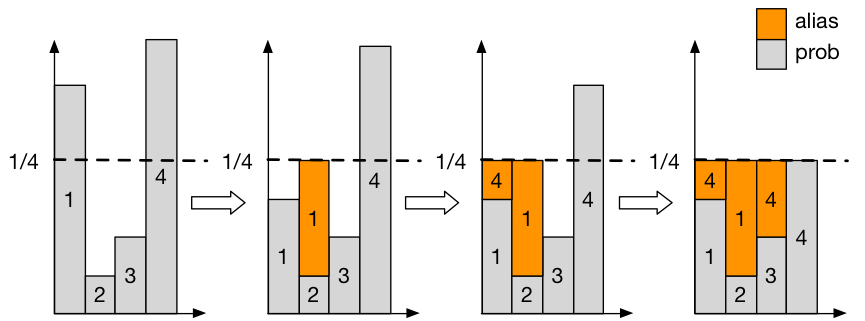
\includegraphics[width=1\linewidth]{alias-table}
\caption{Alias Table构建过程示意}
\label{fig:alias-table}       % Give a unique label
\end{figure}
Alias Table\cite{vose1991a}是一项生成随机数的技术。给定一个概率分布$p(X)$,Alias Table能够按照概率分布$p(X)$以$O(1)$的时间复杂度生成一个随机数$x$。
不妨另$p(X) = \{p_0, p_1, ..., p_n\}$表示在变量$X=\{X_0, X_1, ..., X_n\}$上的分布,其中$\sum_i^n {p_i} = 1, p_i \ge 0$。
那么Alias Table技术等价于一次$O(n)$复杂度的初始化操作和任意次$O(1)$复杂的随机数生成操作。

算法\ref{alg:alias-table}中prob和alias是在Init步骤构建好的两个大小为$n$的表。

\begin{algorithm}[htb]  
\caption{Alias Table} 
\label{alg:alias-table}
\textbf{\underline{Rand:}}
\begin{algorithmic}[1] 
\State $u = Uniform(n)$
\State $j = \lfloor u \rfloor$
\If { $(u - j) \le \mbox{prob}[j]$ }
\Return $j$
\Else
~~\Return $\mbox{alias}[j]$
\EndIf
\end{algorithmic}  
\textbf{\underline{Init:}}
\begin{algorithmic}[1] 
\State l = 0; s = 0
\For{ $j = 0\mbox{ to } n - 1$}
\If{ $p_j > \frac{1}{n}$}
$\mbox{large}[l] = j; l = l + 1$
\Else
~~$\mbox{small}[s] = j; s = s + 1$
\EndIf
\EndFor
\While{ $s\ne 0\mbox{ and }l \ne 0$}
\State $s = s - 1; j = \mbox{small}[s]$
\State $l = l - 1; k = \mbox{large}[l]$
\State $\mbox{prob}[j] = n \times p_j$
\State $\mbox{alias}[j] = k$
\State $p_k = p_k + (p_j - \frac{1}{n})$
\If{ $p_k > \frac{1}{n}$}
$\mbox{large}[l] = k; l = l + 1$
\Else
~~$\mbox{small}[s] = k; s = s + 1$
\EndIf
\EndWhile
\While{ $s > 0$}
$s = s - 1; \mbox{prob}[\mbox{small}[s]] = 1$
\EndWhile
\While{ $l > 0$}
$l = l - 1; \mbox{prob}[\mbox{large}[l]] = 1$ \EndWhile
\end{algorithmic}  
\end{algorithm}  

Init算法实际上是对一个面积为1的区域进行填空的过程。
这种填空方法的思路主要来自于,如果把概率看做长度,变量的宽都为1,
对于均匀分布有所有变量的长度都为$frac{1}{n}$,刚好组成一个面积为1的矩形区域。
相当于将面积1等分为$n$个区间,此时随机选取一个$(0, 1)$之间的值,便能立即确定其属于哪个区间。
但这只是特例,大多数时候有一部分变量的概率不到$\frac{1}{n}$,而另外一部分概率超过了$\frac{1}{n}$,
为了构造上面提到的矩形,Alias Table的算法采取优先填满每个等分区间(每个区间最多被两个随机数占用)的方式,用长板补短板,逐一填空。

如图\ref{fig:alias-table}实际上算法\ref{alg:alias-table}的Init步骤等价于在填写一个面积为1的矩形区域。

(1) 该矩形被等分为$n$份,每一份的面积等于$\frac{1}{n}$。

(2) 等分的$n$个子区域又各自分为prob和alias两部分,也就是$\mbox{len}(\mbox{prob}[i]) +\mbox{len}( \mbox{alias}[i]) = \frac{1}{n}$对于任意$i$都成立。

(3) 对于每个变量$X_i$,面积占比为$\mbox{area}[i] = \mbox{len}(\mbox{prob}[i]) + \sum_{j, alias[j]=i}{\mbox{len}(\mbox{alias[j]})}$。

(4) 对所有变量$X_i$,有$\mbox{area}[i] = p_i$。

\subsection{Light LDA}
Light LDA在Sparse LDA和Alias LDA的基础之上进一步提升了采样的效率。
Light LDA认为提议分布$q(\cdot)$的选择对算法快速收敛到真实LDA后验分布$p(\cdot)$具有重要的意义,
挑选得好的分布能够从两个方面提升采样效率:

(1) 从提议分布$q(\cdot)$中采样的效率要远远高于原分布$p(\cdot)$

(2) 非周期马氏链会迅速收敛到平稳状态

事实上,提议分布$q(\cdot)$的选择也是一个权衡利弊的过程。提议分布$q(\cdot)$和真实分布$p(\cdot)$越接近,则非周期马氏链收敛越快,
但是这么一来从$q(\cdot)$中采样可能和直接从$p(\cdot)$中抽样同样复杂。
反过来,如果选择一个不那么相似的提议分布$q(\cdot)$可以令从$q(\cdot)$效率非常高,但是马氏链收敛的速度可能会变极慢。

为了选择高校的提议分布,使得采样的效率高且马氏链的收敛速度快,Light LDA采取了与Sparse LDA和Alias LDA不同的提议策略,
该策略拥有两个提议分布,并且交替地作为高效率的采样分布。

Light LDA发现公式\ref{eq:sample-prob}中拥有两项,其中一项与文档主题计数$n_{k,d}$有关而与词汇主题计数$n_{k,w}$无关,
另外一项则只和词汇主题计数$n_{k,w}$相关而与文档主题计数$n_{k,d}$无关。
不难推理出,该采样公式中概率密度主要集中在那些词汇主题计数$n_{k,w}$和文档主题计数$n_{k,d}$都比较大的主题。
因此,公式\ref{eq:sample-prob}两项均可以作为较好的主题采样分布的提议分布。

\subsubsection{词汇提议分布}
定义词汇提议分布为:
\begin{equation}
p_w(z = k) \propto \dfrac{n_{k,w} +\eta}{n_{k, \cdot} + V \eta}
\end{equation}
从状态$s$转移到$t$的接受率为:
\begin{equation}
\begin{aligned}
& \alpha_w(z=k) = \min \left\{\dfrac{p(t) p_w(s)}{p(s)p_w(t)}, 1\right\} \\
& \dfrac{p(t) p_w(s)}{p(s)p_w(t)}= \dfrac{ (n_{t,d}^{\neg di} + \alpha)(n_{t,w}^{\neg di} + \eta) (n_{s,\cdot}^{\neg di} + V \eta) (n_{s,w} + \eta) ( n_{t, \cdot} + V \eta)}
{ (n_{s,d}^{\neg di} + \alpha)(n_{s,w}^{\neg di} + \eta) (n_{t,\cdot}^{\neg di} + V \eta) (n_{t,w} + \eta) ( n_{s, \cdot} + V \eta)}
\end{aligned}
\end{equation}
如上,因为在算法中$n_{k, w}$和$n_{k, d}$等计数会被提前计算,并且以常数时间更新,所以接受率$\alpha_w$的计算时间复杂度为$O(1)$。
显然$\pi_w$的值相对来说比较大,每次提议采样$t$都有比较大的概率被接受。
除此之外,Light LDA仍然假设段时间内概率$p_w$不会发生很大的变化,并使用Alias Table技术在每轮迭代之前预先计算好AliasTable来提高采样的速度。

\subsubsection{文档提议分布}
定义文档提议分布为:
\begin{equation}
p_d(z = k) \propto (n_{k,d} +\alpha)
\end{equation}
从状态$s$转移到$t$的接受率为:
\begin{equation}
\begin{aligned}
& \alpha_d(z=k) = \min \left\{\dfrac{p(t) p_d(s)}{p(s)p_d(t)}, 1\right\} \\
& \dfrac{p(t) p_d(s)}{p(s)p_d(t)}=
\dfrac{ (n_{t,d}^{\neg di} + \alpha)(n_{t,d}^{\neg di} + \eta) (n_{s,\cdot}^{\neg di} + V \eta) (n_{s,d} + \eta) }
{ (n_{s,d}^{\neg di} + \alpha)(n_{s,d}^{\neg di} + \eta) (n_{t,\cdot}^{\neg di} + V \eta) (n_{t,d} + \eta) }
\end{aligned}
\end{equation}
和词汇提议分布的定义类似,这里$\alpha_d$的计算时间复杂度也为$O(1)$。

\begin{figure}[htb]\centering
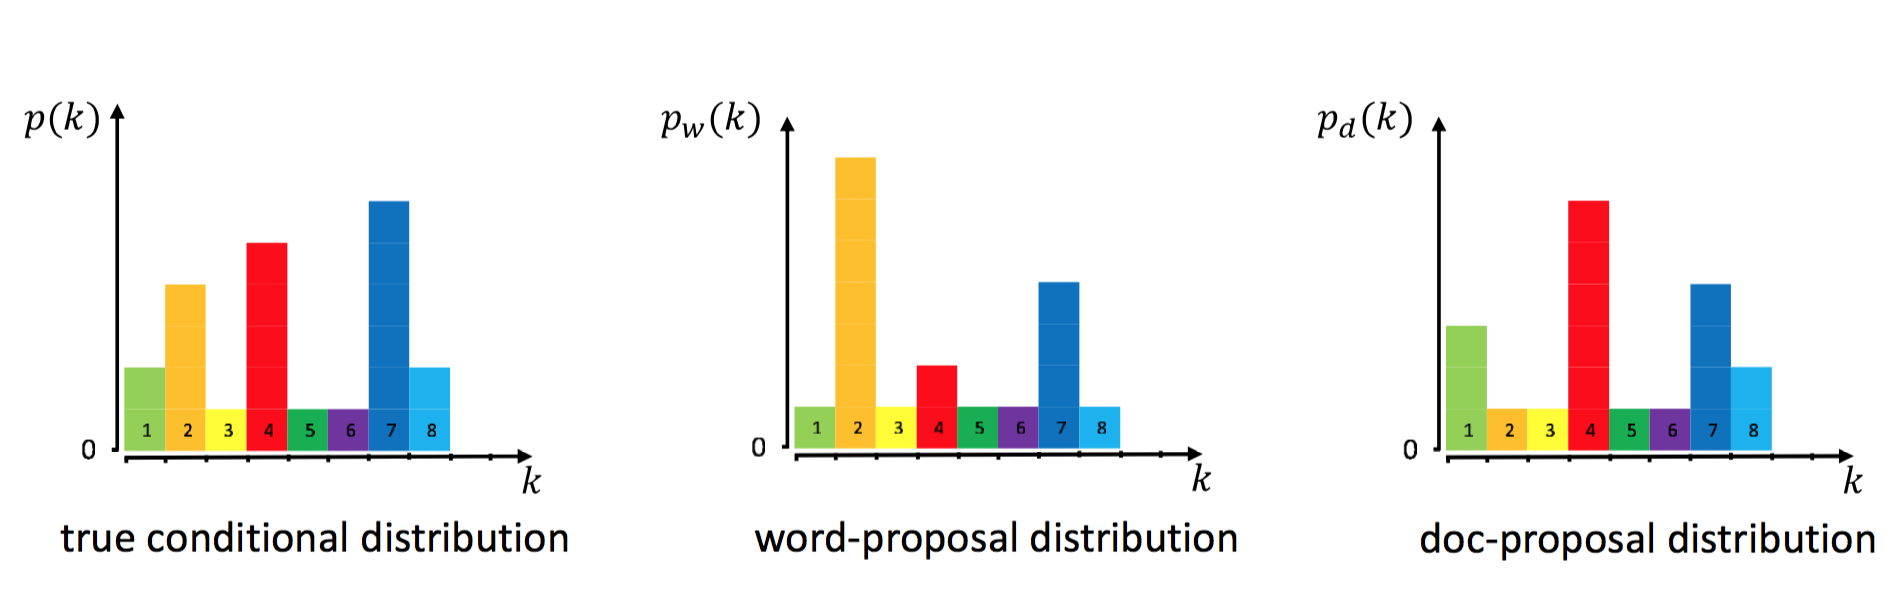
\includegraphics[width=1\linewidth]{mh-proposal}
\caption{提议分布与真实采样分布}
\label{fig:mh-proposal}       % Give a unique label
\end{figure}

如图\ref{fig:mh-proposal},使用原分布$p(k)$算法会倾向于采样得到概率$p_w(k)$和$p_d(k)$双高的主题。
词汇提议分布$p_w(k)$倾向于采样得到当前词汇语义比较集中的主题变量,
而文档提议分布$p_d(k)$倾向于采样得到当前文档语义比较集中的主题变量。
虽然,两者直接有大概率重叠的空间,但是并不是完全相同。
单纯使用词汇提议分布最终会使得词汇主题的分布更加稀疏;
反之,单纯使用文档提议分布最终更会使得文档主题的分布更加稀疏。
但是这两种方法的采样效率都很高——采样复杂度都为$O(1)$。

Metropolis Hastings算法能够快速收敛的关键在于快速地遍历状态空间。
根据上面的分析我们知道,词汇提议分布和文档提议分布都带有倾向性,所遍历的状态子空间不完全重叠。
为了更好地模拟分布$p(k)$,Ligth LDA使用一种循环提议的方式交替地使用词汇提议和文档提议。
相当于得到了一个新的提议:
\begin{equation}
p_c(k) \propto p_w(k) p_d(k)
\end{equation}
该提议兼顾了$p_w(k)$和$p_d(k)$,只有那些$p_w(k)$和$p_d(k)$都比较高的主题才会被频繁地采样。

\section{本章小结}
Sparse LDA利用了主题模型参数的稀疏性来降低了采样的复杂度,而Alias LDA借助Alias和Metropolis-Hastings算法进一步提升了采样的效率。
这类加速技术对主题模型采样的效率具有非常大的意义,因为原先朴素的采样方法的时间复杂度为$O(K)$,时间效率受到了主题变量维度大小的严重限制,
导致了许多时候无法使用高维的特征表达。
Light LDA在Sparse LDA和Alias LDA的基础之上提出了效率更高的采样方案。
在流式主题模型这种对时间效率要求极高的环境下,这些高效的采样方案为本文实时地进行大规模主题参数的采样的可能。

